\documentclass[11pt,a4paper]{article}

% Encoding and typography
\usepackage[T1]{fontenc}
\usepackage[utf8]{inputenc}
\usepackage{lmodern}
\usepackage{microtype}
\usepackage{amsmath,amssymb}
\usepackage{helvet}
\renewcommand{\familydefault}{\sfdefault}

% Page layout
\usepackage[a4paper,margin=22mm,headheight=23pt]{geometry}
\usepackage{setspace}
\setstretch{1.08}
\usepackage{parskip}
\usepackage{ragged2e}

% Graphics and colour
\usepackage{graphicx}
\usepackage[table]{xcolor}
\usepackage{caption}
\usepackage{subcaption}
\usepackage{float}

% Tables
\usepackage{array}
\usepackage{booktabs}
\usepackage{tabularx}

% Headers, links, and headings
\usepackage{fancyhdr}
\usepackage{lastpage}
\usepackage{titlesec}
\usepackage[most]{tcolorbox}
\usepackage{hyperref}
\usepackage{xurl}

\definecolor{UPBlue}{HTML}{003B5C}
\definecolor{UPAccent}{HTML}{C69214}
\definecolor{UPLight}{HTML}{EEF5F8}
\definecolor{TableHead}{HTML}{DCEAF0}
\definecolor{TableRule}{HTML}{6E8FA3}

\hypersetup{
  colorlinks=true,
  linkcolor=UPBlue,
  urlcolor=UPBlue,
  citecolor=UPBlue,
  pdfauthor={Department of Electrical, Electronic and Computer Engineering},
  pdftitle={MPPT Circuit User Manual},
  pdfsubject={Module ENR 420},
  pdfkeywords={MPPT, four-switch buck-boost converter, solar panels, STM32}
}
\urlstyle{same}

\graphicspath{{fig/}}
\captionsetup{font=small,labelfont={bf,color=UPBlue},labelsep=colon,skip=4pt}
\renewcommand{\arraystretch}{1.24}
\setlength{\tabcolsep}{7pt}
\newcolumntype{Y}{>{\RaggedRight\arraybackslash}X}
\newcolumntype{L}[1]{>{\raggedright\arraybackslash}p{#1}}

\titleformat{\section}
  {\Large\bfseries\color{UPBlue}}
  {\thesection}{0.65em}{}
\titleformat{\subsection}
  {\large\bfseries\color{UPBlue}}
  {\thesubsection}{0.65em}{}
\titlespacing*{\section}{0pt}{1.2em}{0.55em}
\titlespacing*{\subsection}{0pt}{1.0em}{0.35em}

\pagestyle{fancy}
\fancyhf{}
\lhead{\small MPPT Circuit User Manual}
\rhead{\small Module ENR 420}
\cfoot{\small Page \thepage\ of \pageref*{LastPage}}
\renewcommand{\headrulewidth}{0.4pt}
\renewcommand{\headrule}{\hbox to\headwidth{\color{UPAccent}\leaders\hrule height \headrulewidth\hfill}}

\newcommand{\code}[1]{\texttt{#1}}
\newcommand{\Vout}{V_{o}}
\newcommand{\Vin}{V_{\mathrm{in}}}

\begin{document}
\hypersetup{pageanchor=false}
\pagestyle{empty}

\begin{titlepage}
  \thispagestyle{empty}
  \centering
  \vspace*{7mm}
  {\Large\bfseries Department of Electrical, Electronic and Computer Engineering\par}
  \vspace{12mm}
  
\includegraphics[width=0.72\textwidth]{up_logo.jpeg}\par
  \vspace{16mm}
  {\Huge\bfseries\color{UPBlue} MPPT Circuit User Manual\par}
  \vspace{4mm}
  {\large Copyright reserved\par}
  \vspace{14mm}
  {\LARGE\bfseries Module ENR 420\par}
  \vfill
  \begin{tcolorbox}[
    colback=UPLight,
    colframe=UPBlue,
    width=0.82\textwidth,
    boxrule=0.9pt,
    arc=1.5mm,
    left=5mm,right=5mm,top=4mm,bottom=4mm]
    \centering
    A concise guide to the MPPT circuit, PCB connections, sensing interfaces, and microcontroller pin mapping used in Practicals 1 and 3.
  \end{tcolorbox}
  \vspace*{10mm}
\end{titlepage}

\thispagestyle{empty}
\tableofcontents
\clearpage
\hypersetup{pageanchor=true}
\pagenumbering{arabic}
\pagestyle{fancy}

\section{Overview}

Maximum power point tracking (MPPT) is necessary to ensure that solar panels can operate at their maximum efficiency and produce maximum possible power under changing conditions. To implement MPPT, a DC-DC converter is required, which can be controlled by a microcontroller running an MPPT algorithm. Students will be provided with a circuit and a microcontroller to use for Practicals 1 and 3. This document will serve as a guide for how to use the circuit.

Figure~\ref{fig:system-block-diagram} shows a block diagram of the overall system, which consists of an MPPT circuit which draws power from the solar panels at the input, and outputs power to a battery and a load. The MPPT circuit outputs the solar panel voltage and current, battery voltage and current, and load current to the microcontroller, which determines the operating point of the system, and controls the circuit using PWM, disable and load enable signals. For Practical 1 and 3, two series connected Model YLM-J 3.0 PRO solar panels will be connected as the input to the circuit. In Practical 3, a particle swarm optimisation (PSO) MPPT algorithm will be implemented on the microcontroller.

\begin{figure}[H]
  \centering
  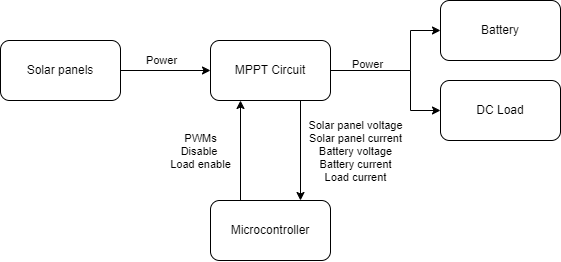
\includegraphics[width=0.86\textwidth]{system_block_diagram.png}
  \caption{System block diagram}
  \label{fig:system-block-diagram}
\end{figure}

\section{Circuit Description}

The DC-DC converter circuit is a four-switch buck-boost (4SBB) converter. The converter can step the input voltage up or down, ensuring that the maximum power point can be tracked for diverse loads, conditions, and solar panel configurations. Compared to a conventional buck-boost converter, the 4SBB provides a non-inverted voltage polarity at the output and achieves higher efficiencies. A basic circuit diagram is shown in Figure~\ref{fig:four-switch-buck-boost}.

\begin{figure}[H]
  \centering
  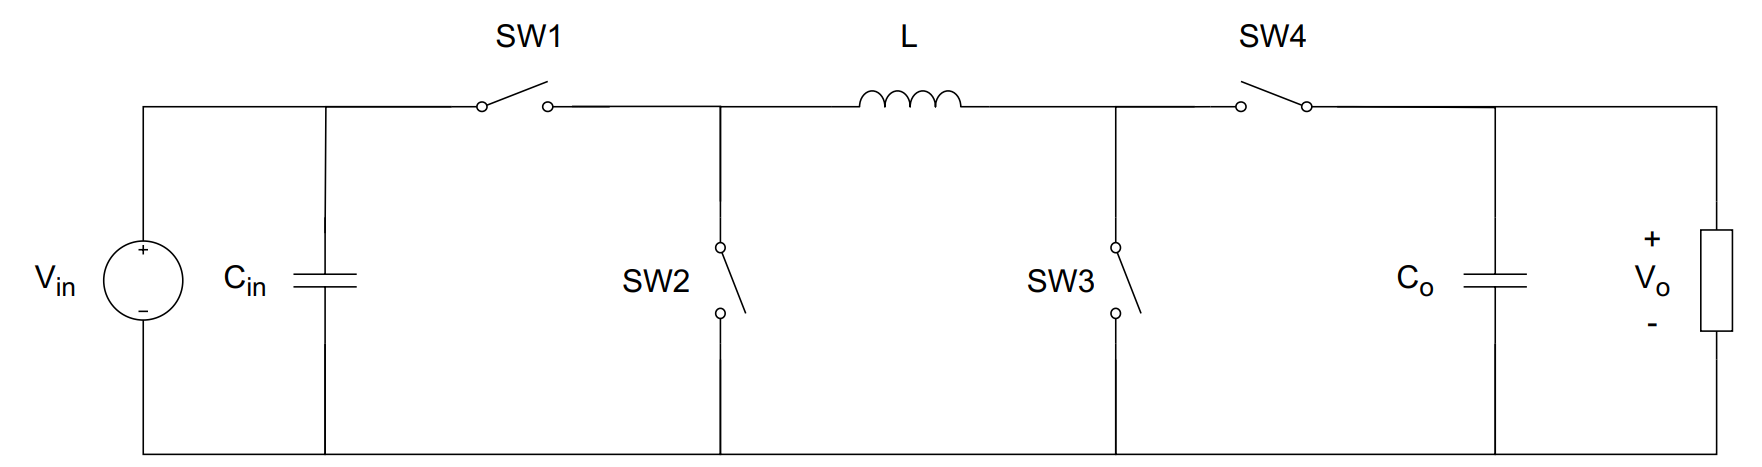
\includegraphics[width=\textwidth]{four_switch_buck_boost.png}
  \caption{Four-switch buck-boost converter circuit diagram}
  \label{fig:four-switch-buck-boost}
\end{figure}

Switch 1 and switch 2 operate with complementary duty cycles of $D_1$ and $1-D_1$ respectively, while switch 3 and switch 4 operate with duty cycles of $D_2$ and $1-D_2$ respectively. Switch 1 and switch 3 operate in phase.

The voltage gain of the converter is given by
\begin{equation}
  \frac{\Vout}{\Vin}=\frac{D_1}{1-D_2}.
  \label{eq:voltage-gain}
\end{equation}

By setting $D_2=0$ (SW4 is closed and SW3 is open), the converter acts as a buck converter with a voltage gain of $D_1$. With $D_1=1$ (SW1 is closed and SW2 is open), the converter acts as a boost converter with a gain of $1/(1-D_2)$. When $D_1=D_2=D$, the converter acts as a buck-boost converter with a gain of $D/(1-D)$. SW1 and SW2 form the buck side of the converter, while SW3 and SW4 form the boost side of the converter.

The maximum voltage and current ratings of the circuit are given in Table~\ref{tab:max-ratings}.

\begin{table}[H]
  \centering
  \caption{Circuit maximum ratings}
  \label{tab:max-ratings}
  \begin{tabularx}{0.70\textwidth}{@{}Y r@{}}
    \toprule
    \rowcolor{TableHead}\textbf{Parameter} & \textbf{Value} \\
    \midrule
    Input voltage  & $100\,\mathrm{V}$ \\
    Input current  & $15\,\mathrm{A}$ \\
    Output voltage & $60\,\mathrm{V}$ \\
    Output current & $25\,\mathrm{A}$ \\
    \bottomrule
  \end{tabularx}
\end{table}

The component values used for the inductor and capacitors are given in Table~\ref{tab:component-values}. The circuit is designed for $250\,\mathrm{kHz}$ switching.

\begin{table}[H]
  \centering
  \caption{Component values}
  \label{tab:component-values}
  \begin{tabularx}{0.70\textwidth}{@{}Y r@{}}
    \toprule
    \rowcolor{TableHead}\textbf{Parameter} & \textbf{Value} \\
    \midrule
    $C_{\mathrm{in}}$ & $25\,\mu\mathrm{F}$ \\
    $L$               & $20\,\mu\mathrm{H}$ \\
    $C_o$             & $15\,\mu\mathrm{F}$ \\
    \bottomrule
  \end{tabularx}
\end{table}

\section{Printed Circuit Board Configuration}

A printed circuit board (PCB) has been designed and manufactured for the MPPT circuit. The circuit includes voltage and current sensors for the input and output. Additionally, the circuit contains auxiliary power supplies to power the sensing circuitry and the microcontroller. The unpopulated PCB is shown in Figures~\ref{fig:pcb-unpop-top} and~\ref{fig:pcb-unpop-bottom}.

\begin{figure}[H]
  \centering
  \begin{minipage}[t]{0.47\textwidth}
    \centering
    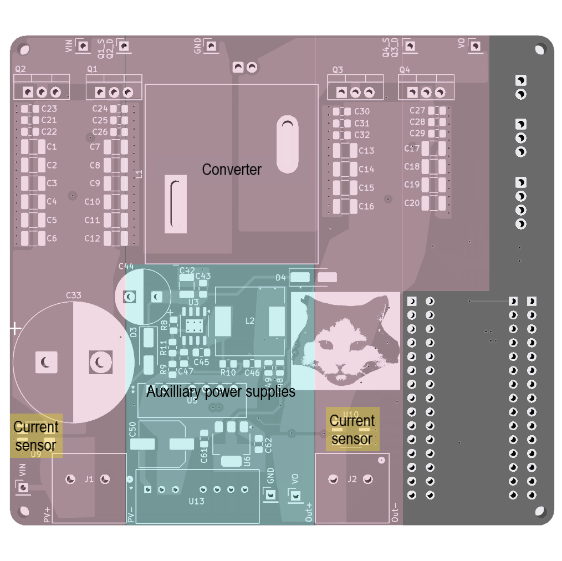
\includegraphics[width=0.92\linewidth]{pcb_unpopulated_top.png}
    \caption{Unpopulated PCB top view}
    \label{fig:pcb-unpop-top}
  \end{minipage}\hfill
  \begin{minipage}[t]{0.47\textwidth}
    \centering
    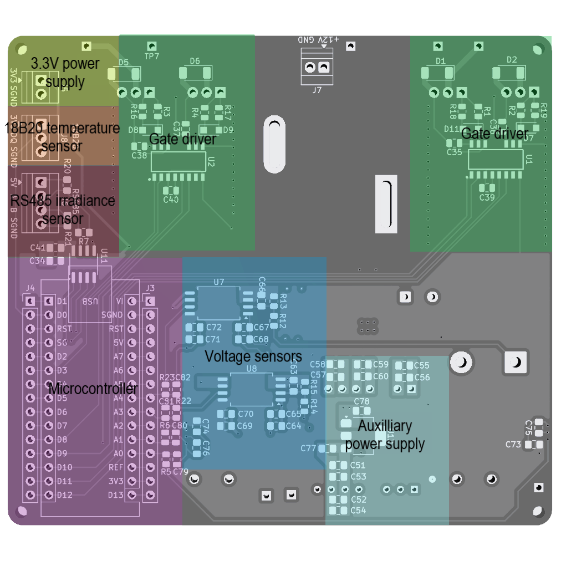
\includegraphics[width=0.92\linewidth]{pcb_unpopulated_bottom.png}
    \caption{Unpopulated PCB bottom view}
    \label{fig:pcb-unpop-bottom}
  \end{minipage}
\end{figure}

The PCB is pictured with components in Figures~\ref{fig:pcb-top-components} and~\ref{fig:pcb-bottom-components}, with connections indicated.

\begin{figure}[H]
  \centering
  \begin{minipage}[t]{0.47\textwidth}
    \centering
    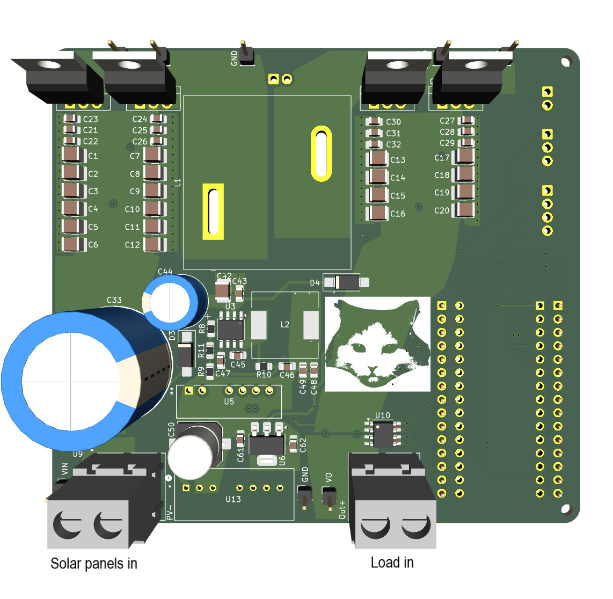
\includegraphics[width=0.95\linewidth]{pcb_top_components.png}
    \caption{PCB top view with components}
    \label{fig:pcb-top-components}
  \end{minipage}\hfill
  \begin{minipage}[t]{0.47\textwidth}
    \centering
    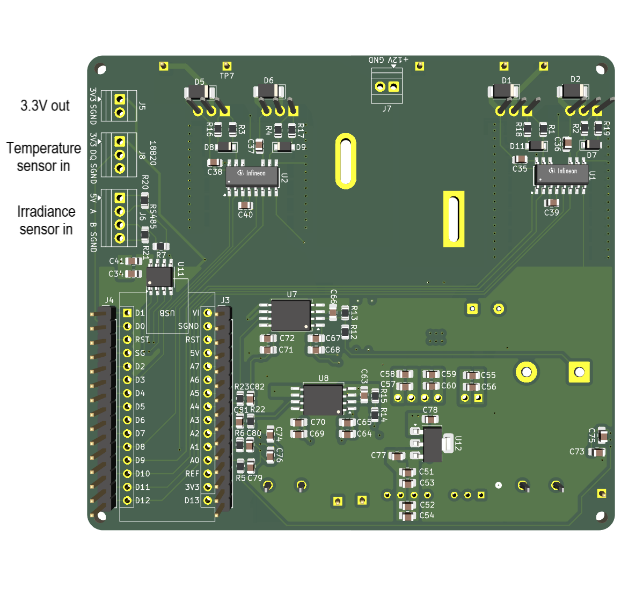
\includegraphics[width=0.95\linewidth]{pcb_bottom_components.png}
    \caption{PCB bottom view with components}
    \label{fig:pcb-bottom-components}
  \end{minipage}
\end{figure}

As can be seen in Figure~\ref{fig:pcb-top-components}, the solar panels must be connected to the screw terminal labelled ``Solar panels in'', and the load can be connected to the screw terminal labelled ``Load in''.

\section{Microcontroller}

A STM32 NUCLEO-F303K8 microcontroller will be provided. The microcontroller can be plugged into headers on the PCB. The microcontroller connections are summarised in Table~\ref{tab:microcontroller-pins}.

\begin{table}[H]
  \centering
  \footnotesize
  \caption{Microcontroller pin connections}
  \label{tab:microcontroller-pins}
  \begin{tabularx}{\textwidth}{@{}L{0.11\textwidth} L{0.20\textwidth} L{0.23\textwidth} L{0.34\textwidth}@{}}
  \toprule
  \rowcolor{TableHead}\textbf{STM pin label} & \textbf{STM pin function} & \textbf{Connection on board} & \textbf{Description} \\
  \midrule
  \code{D1}  & \code{TIM1\_CH2N} & \code{BST\_LOPWM} & Boost side low switch (SW3) PWM \\
  \code{D0}  & \code{GPIO}       & \code{DQ}         & DS18B20 temperature sensor one-wire connection \\
  \code{D3}  & \code{TIM1\_CH2}  & \code{BST\_HIPWM} & Boost side high switch (SW4) PWM \\
  \code{D4}  & \code{UART1\_RX}  & \code{RO}         & ST4E1216IDT receiver data output \\
  \code{D5}  & \code{UART1\_TX}  & \code{DI}         & ST4E1216IDT transmission data input \\
  \code{D6}  & \code{GPIO}       & \code{RE}         & ST4E1216IDT receiver enable input, active low \\
  \code{D7}  & \code{GPIO}       & \code{DE}         & ST4E1216IDT driver enable input, active high \\
  \code{D8}  & \code{GPIO}       & \code{BST\_DIS}   & Boost side gate driver disable \\
  \code{D9}  & \code{TIM1\_CH1}  & \code{BCK\_HIPWM} & Buck side high switch (SW1) PWM \\
  \code{D10} & \code{TIM1\_CH1N} & \code{BCK\_LOPWM} & Buck side low switch (SW2) PWM \\
  \code{D11} & \code{GPIO}       & \code{BCK\_DIS}   & Buck side gate driver disable \\
  \code{D12} & \code{GPIO}       & \code{BCK\_STP}   & Buck side shoot-through protection \\
  \code{D13} & \code{GPIO}       & \code{BST\_STP}   & Boost side shoot-through protection \\
  \code{A0}  & \code{ADC1\_IN1}  & \code{I\_IN}      & Input current sensor \\
  \code{A1}  & \code{ADC1\_IN2}  & \code{I\_O}       & Output current sensor \\
  \code{A3}  & \code{ADC2\_IN1}  & \code{V\_O}       & Output voltage sensor \\
  \code{A4}  & \code{ADC2\_IN2}  & \code{V\_IN}      & Input voltage sensor \\
  \bottomrule
  \end{tabularx}
\end{table}

\subsection{Gate Drivers}

Two \href{https://www.infineon.com/assets/row/public/documents/24/49/infineon-2edb8259y-datasheet-en.pdf}{2EDB8259Y} half bridge gate drivers are used to drive the buck and boost side of the converter. The buck and boost sides of the converter each have connections for their disable, high-side and low-side PWM, and shoot-through protection pins. When the disable pin is high, switching is disabled. Dead times of $100\,\mathrm{ns}$ are recommended.

\begin{figure}[H]
  \centering
  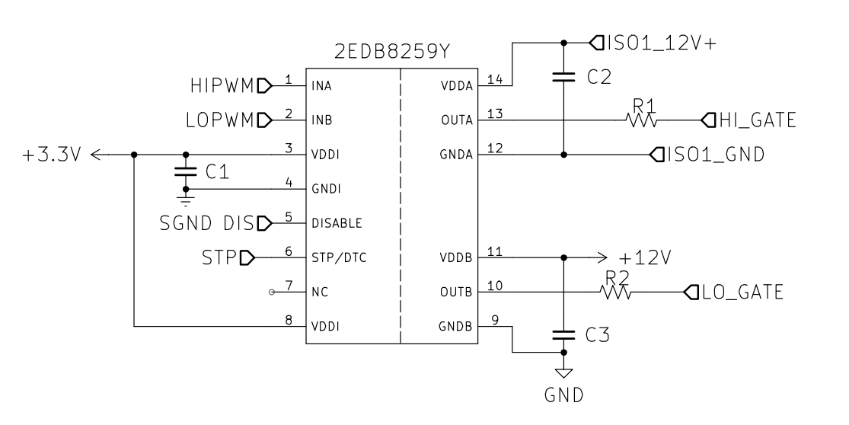
\includegraphics[width=0.76\textwidth]{gate_driver_schematic.png}
  \caption*{2EDB8259Y half bridge gate driver schematic}
  \label{fig:gate-driver-schematic}
\end{figure}

\subsection{Voltage Sensors}

Two \href{https://www.ti.com/product/AMC0311S}{AMC0311S} isolated amplifiers are used for sensing the input and output voltages. The circuit schematic can be seen in Figure~\ref{fig:voltage-sensor}.

\begin{figure}[H]
  \centering
  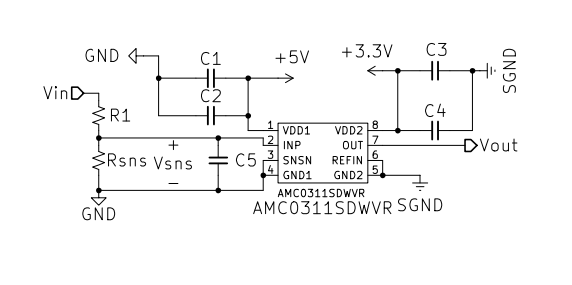
\includegraphics[width=0.70\textwidth]{amc0311s_voltage_sensor.png}
  \caption{AMC0311S voltage sensor}
  \label{fig:voltage-sensor}
\end{figure}

The output, $V_{\mathrm{out}}$, is connected to \code{ADC2\_IN2} and \code{ADC2\_IN1} for the input and output voltages respectively.

\begin{table}[H]
  \centering
  \caption{Voltage sensor parameter values}
  \label{tab:voltage-sensor-values}
  \begin{tabularx}{0.76\textwidth}{@{}Ycc@{}}
    \toprule
    \rowcolor{TableHead} & \textbf{Input voltage sensor} & \textbf{Output voltage sensor} \\
    \midrule
    \textbf{$R_1$ ($\mathrm{k}\Omega$)}        & 100 & 100 \\
    \textbf{$R_{\mathrm{sns}}$ ($\mathrm{k}\Omega$)} & 2.2 & 3.6 \\
    \bottomrule
  \end{tabularx}
\end{table}

\subsection{Current Sensors}

Two Allegro MicroSystems \href{https://www.allegromicro.com/-/media/files/datasheets/ct416-datasheet.pdf}{CT416} magnetoresistive current sensors are used for input and output current sensing. A CT416-HSN820DR unidirectional $20\,\mathrm{A}$ current sensor is used to measure the input current, and a CT416-HSN830MR bidirectional $30\,\mathrm{A}$ current sensor is used to measure the output current. The outputs are connected to \code{ADC1\_IN1} and \code{ADC1\_IN2} for the input and output current sensors respectively.

\begin{figure}[H]
  \centering
  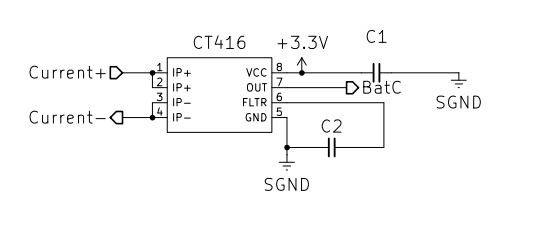
\includegraphics[width=0.62\textwidth]{ct416_current_sensor.png}
  \caption{CT416 current sensor}
  \label{fig:current-sensor}
\end{figure}

\subsection{Temperature Sensors}

\subsection{Irradiance Sensor}

A \href{https://wiki.dfrobot.com/sen0640/}{RS485 Photoelectric Solar Radiation Sensor} will be provided for solar irradiance sensing. This can be plugged into screw terminal \code{J8}, which connects it to a \href{https://www.digikey.co.za/en/products/detail/stmicroelectronics/ST4E1216IDT/22971696}{ST4E1216IDT} for RS485 to UART signal conversion.

\end{document}
